\documentclass[12pt,a4paper]{article}
\usepackage{graphicx}
\usepackage{url}

\begin{document}

\begin{titlepage}

\center{\Huge{The Black Box}}
\center{\large{Perception in the 19th century}}
\vspace{1cm}

\begin{figure}[h]
	\centering
	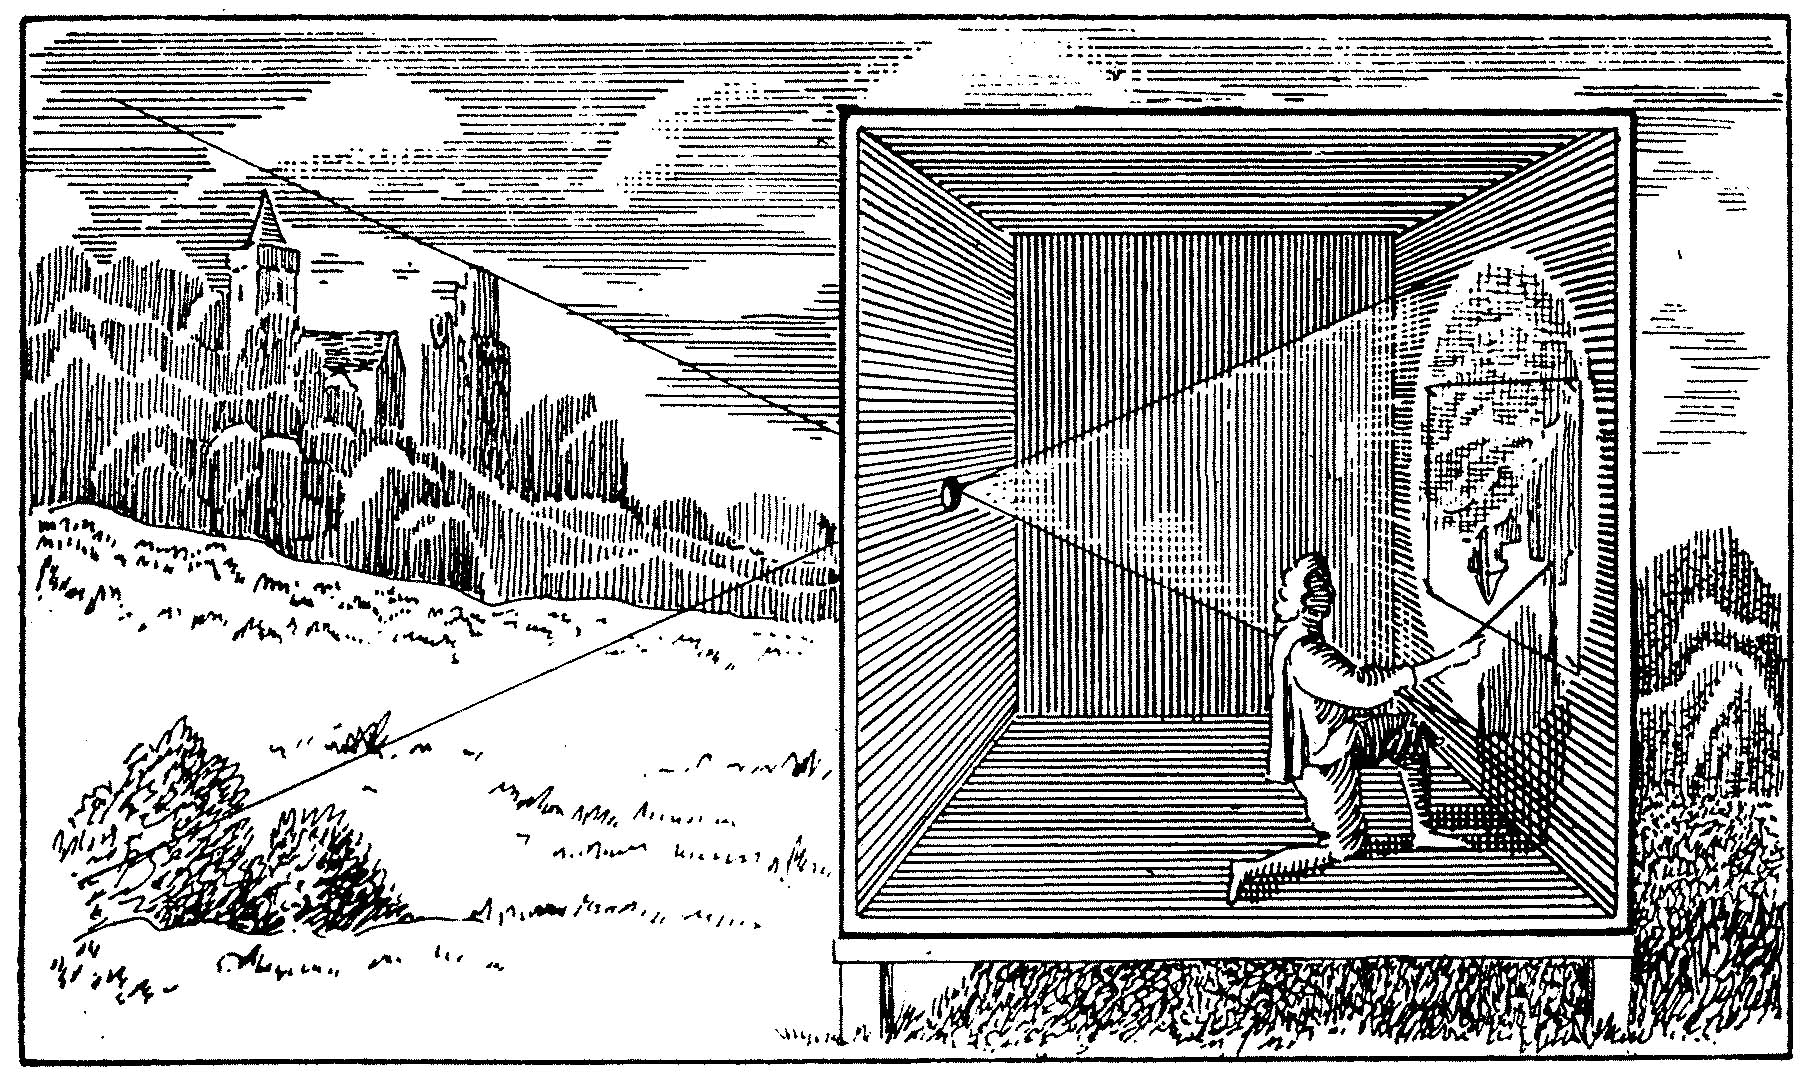
\includegraphics[width=\textwidth]{img/cameraobscura.jpeg}
\end{figure}

\vspace{1cm}
\center{Dominik Schlegel}
\center{\today}

\end{titlepage}


\newpage

\section*{Preface}

On the following pages I will discuss the development of the human perception model and its
inseparable relations to the scientific body in the 19th century. The essay focusses on
{\it{Subjective Vision and the Separation of the Senses}} \cite{crary} and includes information from
{\it{Techniques of the Observer}} \cite{crary}, {\it{The Images of Precision: Helmholtz and the
graphical Method in Physiology}} \cite{holmes} and {\it{Camera and Mind}} \cite{ellenbogen}. Basic
knowledge of the material is assumed and only the key points will be repeated in order to explain
my view.

As an additional, diverse source I picked a topic about the beginning of the institutionalization of people
with disabilities during the 19th century and its direct connection to the respective idea of
perception and human society \cite{earlymovement}.

\section*{Thesis}

I claim that the change from the 18th centuries humanly passive and pseudo-objective
perception to the physiologically objective perception of the 19th century was crucial in order to
enable the massive growth in production of scientific knowledge during the 19th century.
The human body was far from being completely understood at the end of the 18th century but
nevertheless people took perceived impressions as the undiluted, completely clear representation of
their true nature.
This premise reduces the observer to a simple, passive receiver of information without any transformation
of the input from outside - which is not entirely true as we know nowadays.
One can easily think about the numerous possible conflicts resulting from parties with differently developed
senses (e.g. eyesight).

At the same time researches started to play around with the senses and challenged this humanly passive model
of perception. As a result people became unsure about the intake of their senses and the human body
manifested itself as the nature of perception (from physics to physiology). The human body can therefore be
seen as a black box, an object in which we do not not what is going on but in which we expect a
transformation of the input. The step to the acceptance of this black box is of prime importance to me.
Having the black box model researchers could start to quantify perception and get closer to truth
representations of nature.

Additionally one should not forget the inherent link between the new model of perception and human society.
The researchers pursuing this model of perception had many contestants and had a hard time publishing
their findings in the beginning of the physiological movement.

\newpage

Relating to my second source, people whose senses were non- or malfunctional were not able to perceive nature
based on the humanly passive model - and as a consequence were not accepted by the broad human society. This
changed with the model of perception, whereas it became clear that every human transforms nature and
therefore nobody can tell the actual truth of an occurrence. I do not say that this was the major reason for
rise of the institutionalization of people with disabilities but it certainly did play its part.

\section*{Reading}

{\it{Subjective Vision and the Separation of the Senses}} is a chapter of the book {\it{Techniques of the
Observer}} \cite{crary} written by Jonathan Crary. The essay is composed upon a literature collection and
refers to various famous historical figures. The two major topics discussed are the rise of physiology and
the establishment and reframing of new sciences.

In the following sections I will cover the main aspects of the reading and relate them to my Thesis.
Since the topics sometimes overlap with sections discussed in other readings, I will include that
information and mention the respective sources.

\subsection*{Camera Obscura and Subjective Vision}

The camera obscura is an optical device based on the principle of the pinhole camera model \cite{camera}. While
the principle has been known to mankind since approximately 400 BCE, a sufficiently precise realization of the
camera obscura was not achieved until the end of the 16th century. In the 17th century more people began to
work with the device and some started to develop theories about its relation to the human observer.

One of them was Isaac Newton who showed that a ray of white light - the portion of light passing through the
inlet of the camera obscura could be separated into the rainbow colors by using a prism \cite{newtongoethe}.
Newton published his findings in his major work: {\it{Opticks or a treatise of the reflections, refractions,
inflections andcolours of light}} \cite{opticks}.
It is important to note that the influence of physiology on perception
was not part of Newton's studies. The camera obscura established unclouded relations between
the artificial world inside the box and the natural world outside and enabled a clear separation
and definition of object and observer. The observer himself was not of interest for Newton and therefore the
possible correctness of observations was not challenged nor verified in terms of quality.

\newpage

Over a hundred years later Johann Wolfgang von Goethe made the camera obscura the site of his optical studies
as well. Goethe summarises his work in {\it{Farbenlehre}} \cite{farbenlehre}. 
Goethe denied and battled Newton's theories about white light. For Goethe white light was the visible
absence of color whereas for Newton white light was the sum of all colors - this is a crucial difference
with correspondingly diverse resulting theories. As we know by today Newton was right, but at that time it
was not clear which theory is correct and Goethe made important discoveries, even though he seemed to be on
the wrong path from the start.

In contrast to Newton, Goethe started to involve physiology in his optical studies. This is the point where
the question of the human black box will turn up. Goethe created the perfect scenario for displaying the
physiological effects on the sense of sight and therefore on the observer by only a minimal modification of the
camera obscura: Goethe sealed the hole after a short aperture time.

The observer could now still experience an image even thought there was no
light source present. This contradicts the logic behind an observer seeing only real objects visible to him.
The resulting shift from a constant, passive, objective observer to a physiologically active, subjective
observer defines the human body as the active producer of an optical experience and as a direct
consequence, of all sensory experiences.
Thanks to this step the existence of a black box, the human perception as an active system became
undeniable. One speciality about Goethe's observer model is the inseparability of two models usually
presented as distinct and contradictory: the observer as a strictly physiological system and the
autonomous, independent producer of his/her own experiences.

At the same time other researchers such as Immanuel Kant strengthen this change of the point of view
in vision with their discoveries. William Blakes agrees on the model and Michel Foucault
emphasizes the the inconsistent relation to the old model.

Goethe and other researchers continued working with the sense of sight and began to discover
properties of the black box.
This means that the human itself started to examine the complex properties of its perception
in form of a legion of researchers for the first time. Because of the complexity of this topic
straight and efficient progress is not expected and researchers had numerous conflicts with
their colleagues in certain fields. Even though the conflicts slowed down the derivation of a
universal model, they guaranteed the maximum variety of studies to select from.

Later on Arthur Schopenhauer came up with heavily physiological theories on the subject. Schopenhauer
abandoned the combination of the two models Goethe used for his observer. According to Schopenhauer
the experience of color could only result from physiological phenomena. Even thought they disagreed on
that specific topic, both of them were against the Newtonian optics.


\newpage

\bibliographystyle{unsrt}
\bibliography{references.bib}

\end{document}
